Building upon Davis et al, a two dimensional factory was used in this work. The height of the factory was set to 0.768 mm while the width was fixed at 1.536 mm. The total number of producer and vascular cells were 4200 and 1800, respectively where vascular cells contributed to 30 per cent of total number of cells. A total of 384 circulatory cells simulating the external delivery and product extraction system existed as two identical columns on two sides of the factory. The number of all mentioned cells were kept constant through the experiment. The simulations started with a random distribution of producer and vascular cells inside the factory. After 16 simulation hours, the factory started the production phase provided the existence of a network of vascular cells. The aggregate product amount collected by the vascular network and circulatory columns was output after 2 simulated hours as the final throughput of the system. 
\\
\\
A genetic algorithm with a population of 3 chromosomes over an evolution of 500 steps was used for obtaining the optimal values for the seven mentioned parameters. 
\\
\\
Figure 1 shows the throughput of our cell factory during the evolution of this genetic algorithm. After 500 sweep iterations, the highest total product of the factory reached 616.65788 ug. The parameter values contributing to the best case are shown in Table 1. The factory related to these parameters is depicted in figure 2. 

\begin{figure}[!t]
\centering
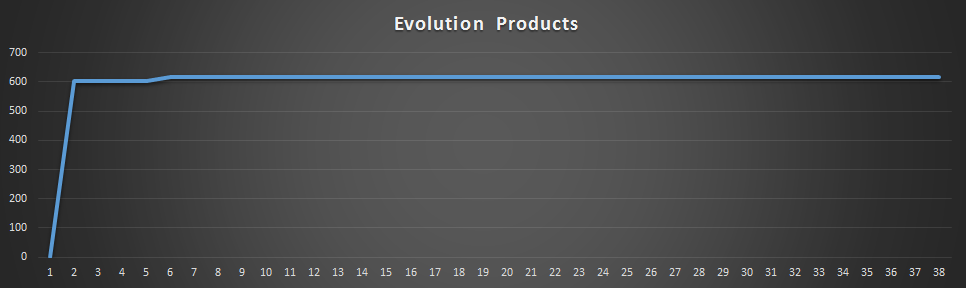
\includegraphics[width=3in]{./figures/sima/results/evolution products.png}

\caption{The amount of product values $Product$ with evolution number $It$}
\label{product}
\end{figure}          

\begin{table}[!t]
\renewcommand{\arraystretch}{1.3}
\caption{The best parameter values the genetic algorithm has identified}
\label{parameter_table}
\centering
\begin{tabular}{c||c}
\hline
\bfseries Parameter & \bfseries Value\\
\hline\hline
\\
\hline
Chemotactic Strength With Gradient & 2.34110242590437\\
\hline
Vascular Cells' Production Rate & 6.1583863371631\\
\hline
Circulatory Cells' Production Rate & 4.26190176330675\\
\hline
Vascular Cells' Chemo-attractant Decay Rate & 0.00839922309567474\\
\hline
Circulatory Cells' Chemo-attractant Decay Rate & 0.0000282503099488372\\
\hline
Vascular Cells' Half-saturation Rate & 0.0092723921166939\\
\hline
\end{tabular}
\end{table}

\begin{figure}[!t]
\centering
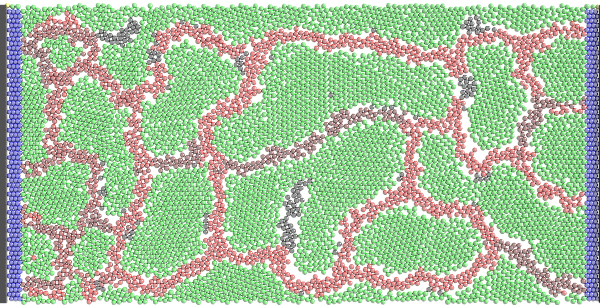
\includegraphics[width=3in]{./figures/sima/results/highest product factory.png}

\caption{The factory with the highest throughput which was found by the GA}
\label{factory}
\end{figure}   